\section{Esecuzione}

L'impianto usato è del tutto analogo a quello costruito nelle esperienze precedenti e presentava
un bypass utile ad isolare la pompa turbomolecolare dal resto dell'impianto. (vedi Figura \ref{fig:impianto})

Poiché la pompa turbomolecolare ha bisogno di una decina di minuti per fermarsi abbiamo cominciato le misure con la pompa rotativa,
misurando solo in un secondo momento la velocità di pompaggio della turbomolecolare.

In questa prima fase abbiamo acceso solo la pompa rotativa e per calcolarne la velocità di pompaggio della pompa rotativa, ci siamo mossi come segue:

\begin{enumerate}
	\item{Abbiamo chiuso la valvola gate alla bocca della turbomolecolare, lasciando aperta la valvola al fondo della stessa,
        in modo che anche l'aria all'interno della pompa venisse rimossa. In questo modo abbiamo evitato perdite
        all'interno dell'impianto stesso;}
	\item{Grazie al bypass abbiamo svuotato tutto l'impianto fino alla pressione limite della pompa rotativa,
        cioè una pressione di qualche Pascal;}
	\item{Successivamente abbiamo prodotto, mediante l'utilizzo della valvola a spillo un flusso
        costante di gas all'interno della camera da vuoto. Questo è stato possibile girando un numero opportuno
        di volte la vite micrometrica della valvola. I flussi per vari valori di apertura sono stati calcolati nella precedente
        esperienza;}
	\item{Quindi grazie al sistema di acquisizione dati, è stato registrato l'andamento della pressione interna alla
        camera in funzione del tempo.  Si è atteso che il valore di pressione all'interno della camera si
        stabilizzasse su un valore costante. Infatti occorre aspettare che la camera raggiunga l'equilibrio
        dopo che è stato variato il flusso in ingresso;}
	\item{Si sono ripetuti i passi 3) e 4) per tutti i valori di flusso da misurare.}
\end{enumerate}

Per calcolare la velocità di pompaggio della pompa turbomolecolare abbiamo seguito lo stesso procedimento
descritto sopra fatta eccezione che in questo caso il baypass era chiuso. In tal caso
si è portata la camera al vuoto limite della turbomolecolare prima di iniziare le misure.

Un'altra differenza tra le procedure seguite per le differenti pompe risiede nei flussi che abbiamo deciso di misurare.
Mentre nel caso della pompa rotativa abbiamo misurato le pressioni limite aprendo la valvola a spillo da 4 a 9 giri,
per la pompa turbomolecolare siamo partiti da un solo giro fino a 6 giri di valvola.
La pompa rotativa ha infatti una pressione di vuoto limite alta, che non avrebbe permesso
una corretta misura della velocità di pompaggio per flussi troppo piccoli (come si vede bene dal grafico
riportato in Figura \ref{fig:rotativa}), come quelli ottenibili al di sotto dei 4 giri della valvola a spillo.
La turbomolecolare, invece, deve lavorare in regimi molecolari, e non ci siamo fidati ad aprire la valvola più di 6 giri.
Un flusso in ingresso troppo alto può infatti danneggiare la pompa. 

\begin{figure}[b!]
	\centering
		\includegraphics[width = 145mm]{rotativa.pdf}
	\caption{Il grafico mostra i valori elaborati della velocità di pompaggio della pompa rotativa in funzione della pressione limite raggiunta in camera. L'asse delle ascisse ha scala logaritmica mentre l'asse delle ordinate ha scala lineare. La velocità di pompaggio, ridotta a basse pressioni, aumenta e si stabilizza all'aumentare della pressione. Questo ha senso, poiché la pompa rotativa funziona bene in regimi viscosi, mentre a pressioni basse il gas è troppo rarefatto, e la pompa diventa poco efficiente.}
		\label{fig:rotativa}
\end{figure}

Sottolineiamo che per misurare la pressione in camera, quando era in azione la pompa turbomolecolare,
non ci siamo più potuti avvalere del sistema di aquisizione dati informatizzato, connesso ai vacuometri Pirani,
in quanto le pressioni raggiunte erano al di fuori del range operativo dello strumento. Si è quindi douto utilizzare
il vacuometro a catodo freddo (Penning) e l'acquisizione delle misure è stata eseguita manualmente. Abbiamo aspettato che la
pressione in camera si stabilizzasse prima di annotare il valore.

\section{Analisi dati}

Le condizioni ambientali presenti durante lo svolgimento di questa sessione di laboratorio sono le seguenti:
tra le ore 14:00 e le 18:00 la temperatura e passata da 25$^\circ$ C a 27$^\circ$ C mentre la pressione atmosferica
è rimasta stabile attorno ad un valore di circa $9.84 \cdot 10^4\, \si{\Pa}$

Grazie all'esperienza di laboratorio precedente, durante la quale abbiamo tarato la valvola a spillo,
conosciamo il flusso di gas in ingresso alla camera da vuoto per alcuni valori di apertura della valvola.
Pertanto per ricavare la velocità di pompaggio delle nostre pompe ci avvaliamo della seguente relazione:

\begin{equation}
	S \,=\, \frac{Q}{P}
\end{equation}
%
dove $S$ rappresenta la velocità di pompaggio, $Q$ il flusso di gas in entrata nella camera da vuoto e $P$ la pressione in camera.
Abbiamo poi confrontato i valori relativi alle velocità di pompaggio da noi ottenuti con quelli forniti dai costruttori.
I manuali riportano una velocità di pompaggio di $S\ped{r} = \SI{7.5}{\cubic\metre\per\hour} = \SI{2}{\cubic\deci\metre\per\second}$
per la pompa rotativa e di $S\ped{t} = \SI{60}{\cubic\deci\metre\per\second}$ per la turbo.

I dati calcolati con l'equazione precedente sono riportati in Tabella \ref{tab:speed}.
Nel caso della rotativa si vede che, a 7, 8 e 9 giri di apertura della valvola, la velocità di pompaggio è vicina a quella riportata
nel manuale. Anche nel caso della turbo, la velocità di pompaggio a pressione alte si avvicina abbastanza a quella riportata nel manuale.
I grafici in Figura \ref{fig:rotativa} e in Figura \ref{fig:turbo}, sono un aiuto grafico alla lettura della tabella, e mostrano,
rispettivamente, le velocità di pompaggio in funzione della pressione per la rotativa e per la turbo.

Tuttavia, i valori da noi trovati risultano essere inferiori, a volte anche in modo significativo,
rispetto alle velocità di pompaggio di riferimento. Tra i motivi che possono incidere su
queste discrepanze fra i valori misurati e quelli del manuale, abbiamo ipotizzato che i più rilevanti siano:

\begin{table}
    \begin{tabular}{l c c c}
        \toprule
        Nr. giri & Q & $S\ped{rotativa}$ & $S\ped{turbo} \\
        \midrule
        1
        2
        3
        4
        5
        5.2
        5.4
        5.6
        5.8
        6
        7
        8
        9
        \bottomrule
    \end{tabular}
\end{table}




\begin{itemize}
    \item{A basse pressioni le pompe non lavorano al massimo della loro velocità di pompaggio poiché i gas sono rarefatti.
        Questo si può vedere considerando per esempio il grafico della pressione nel tempo di una pompa in funzione:
        la forma è quella di un esponenziale negativo. Man mano che ci si avvicina alla pressione limite, la pompa rimuove
        sempre meno aria per ogni ciclo. Bisogna comunque considerare il fatto che a pressioni più basse la stessa quantità di gas
        occupa più volume. Tuttavia ogni pompa ha dei limiti di funzionamento e richiede che la pressione sia al di sopra di un
        certo valore per funzionare in piena efficienza.}
	\item{L'usura della pompa stessa porta ad una minore efficienza dopo un certo periodo di tempo. Le pompe che abbiamo
        usato sono sicuramente ``non nuove'', per usare un eufemismo;}
	\item{I valori forniti dal costruttore si riferiscono alla velocità di pompaggio alla bocca della pompa e non tengono
        conto della conduttanza delle canalizzazioni tra i vari componenti dell'impianto da vuoto. Tale differenza è
        particolarmente evidente soprattutto per la pompa rotativa. Infatti quest'ultima, al contrario della pompa
        turbomolecolare, non era collegata direttamente alla camera da vuoto, ma era connessa tramite un tubo di
        circa un metro di lunghezza;}
\end{itemize}

\begin{figure}[h!]
	\centering
		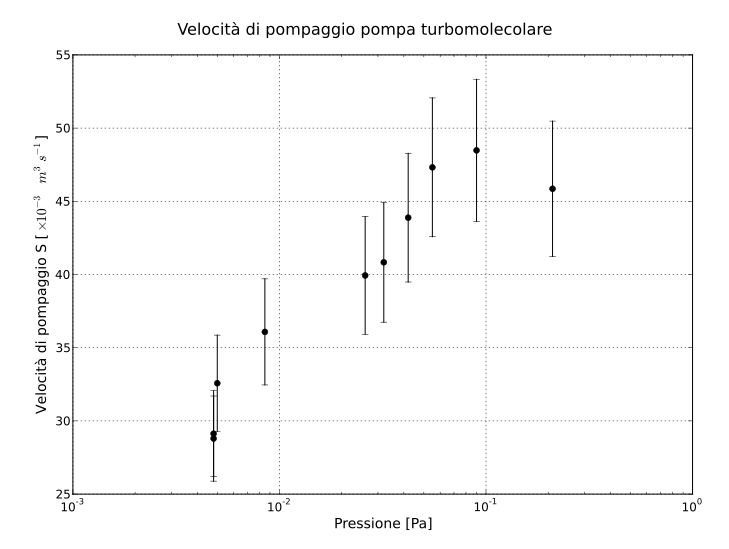
\includegraphics[width=145mm]{turbo.pdf}
	\caption{Il grafico mostra i valori elaborati della velocità di pompaggio della pompa turbomolecolare in funzione della pressione limite raggiunta in camera. L'asse delle ascisse ha scala logaritmica mentre l'asse delle ordinate ha scala lineare.}
		\label{fig:turbo}
\end{figure}
